\documentclass[12pt]{beamer}

% for themes, etc.
\mode<presentation>
{ \usetheme{Copenhagen}
  \usecolortheme{seahorse}{}
}
\setbeamertemplate{itemize items}[default]
\setbeamertemplate{enumerate items}[default]
\setbeamertemplate{navigation symbols}{}

\usepackage{times}  % fonts are up to you
\usepackage{proof}
\usepackage{listings}
\usepackage{courier}
\usepackage{graphicx}
\usepackage{stmaryrd}

\lstset{columns=fullflexible}
\lstset{
  literate={->}{$\to$ }{1}
           {=>}{$\Rightarrow$ }{1}
           {:E}{$\in$ }{1}
           {[|}{$\llbracket$ }{1}
           {|]}{$\llbracket$ }{1},
  escapeinside=||,
  moredelim=**[is][\color{red}]{@}{@},
}
\lstset{language=Haskell}

% these will be used later in the title page
\title{Programming in Vinyl}
\author{Jon Sterling\\
    FOBO
}

\begin{document}

% this prints title, author etc. info from above
\begin{frame}
\titlepage
\end{frame}

\section{Extensible Records and Row Polymorphism}

\begin{frame}
  \frametitle{Records in GHC 7.8}
  Haskell Records are nominally typed. \pause
  \[
    \infer{
      \Gamma\nvdash x : N.T
    }{
      \Gamma\vdash M.S \leadsto \{ \vec{rs} \} &
      \Gamma\vdash N.T \leadsto \{ \vec{rs} \} &
      \Gamma\vdash x : M.S
    }
  \]
\end{frame}

\begin{frame}[fragile]
  \frametitle{Records in GHC 7.8}
  Records may not share field names. \pause

  \begin{lstlisting}
    data R = R { x :: X } |\pause|
    data R' = R' { x :: X } -- ^ Error
  \end{lstlisting}
\end{frame}

\begin{frame}
  \frametitle{Records in GHC 7.8}
  \only<1>{Records are...}
  \only<2>{\Large\centerline{anticompositional}}
\end{frame}

\begin{frame}
  \frametitle{Records in Standard ML}
  \pause
  \Large\centerline{slightly better}
\end{frame}

\begin{frame}[fragile]
  \frametitle{Records in Standard ML}
  \pause
  Records are permutative, and not nominal.\pause
  \[
    \infer{\Gamma\vdash x:\{\vec{ts}\}}{
      \Gamma\vdash x:\{\vec{ss}\} &
      \Gamma\vdash ts\in\mathsf{permutations}(\vec{ss})
    }
  \]
\end{frame}

\begin{frame}
  \frametitle{Records in OCaml}
  \only<1-4> {
  OCaml records are\pause
  \begin{itemize}
    \item structural\pause
    \item endowed with a subtyping relation\pause
    \item but more importantly...
  \end{itemize}
  }
  \only<5>{
    \Large\centerline{row polymorphic}
  }
\end{frame}

\begin{frame}
  \frametitle{Row Polymorphism}\pause
  How do we express the type of a function which adds a field to a record?\pause
  \only<2>{
    \[
      \infer{ f(x) : \{a:A, b:B\} }{ x : \{a:A\} }
    \]
  }
  \only<3>{
    \Large\centerline{NOPE}
  }
  \only<4>{
    \[
      \infer{ f(x) : \{a:A, b:B; \vec{rs}\} }{ x : \{a:A; \vec{rs}\} }
    \]
  }
\end{frame}

\begin{frame}
  \frametitle{Row Polymorphism}\pause
  \begin{itemize}
    \item supports type inference\pause
    \item is compositional\pause
    \item is \textbf{modular}\pause
  \end{itemize}
\end{frame}

\begin{frame}[fragile]
  \frametitle{Roll Your Own in Haskell}\pause
  \begin{lstlisting}
    data (s :: Symbol) ::: (t :: *) = Field |\pause|

    data Rec :: [*] -> * where |\pause|
      RNil :: Rec '[] |\pause|
      (:&) :: !t -> !(Rec rs) -> Rec ((s ::: t) ': rs)

    |\pause|
    class s :E (rs :: [*])|\pause|
    (=:) : s ::: t -> t -> Rec '[s ::: t]|\pause|
    (<+>) : Rec ss -> Rec ts -> Rec (ss ++ ts)
  \end{lstlisting}
\end{frame}
\begin{frame}
  \frametitle{Roll Your Own in Haskell}\pause
  \[
    \infer{
      f\, x :: (\text{"a"} ::: A\in\vec{rs}, \text{"b"} ::: B\in\vec{rs}) \implies \mathsf{Rec}\ \vec{rs}
    }{
      x :: \text{"a"} ::: A\in\vec{rs}\implies \mathsf{Rec}\ \vec{rs}
    }
  \]
\end{frame}

\section{Universes \`a la Tarski}

\begin{frame}
  \frametitle{Universes \`a la Tarski}\pause
  \begin{itemize}
    \item A type $\mathcal{U}$ of \textbf{codes} for types.
      \pause
    \item Function $\llbracket-\rrbracket_\mathcal{U} : \mathcal{U}\to\mathbf{Type}$.
      \pause
      \[
        \infer{
          \Gamma\vdash\llbracket s\rrbracket_\mathcal{U} : \mathbf{Type}
        }{
          \Gamma\vdash s : \mathcal{U}
        }
      \]
    \pause
    \item The Tarski universe $\mathcal{U}$ is a set, but the ambient universe $\mathbf{Type}$ may not necessarily be.
  \end{itemize}
\end{frame}

\begin{frame}
  \frametitle{Universes \`a la Tarski}
  \begin{center}
    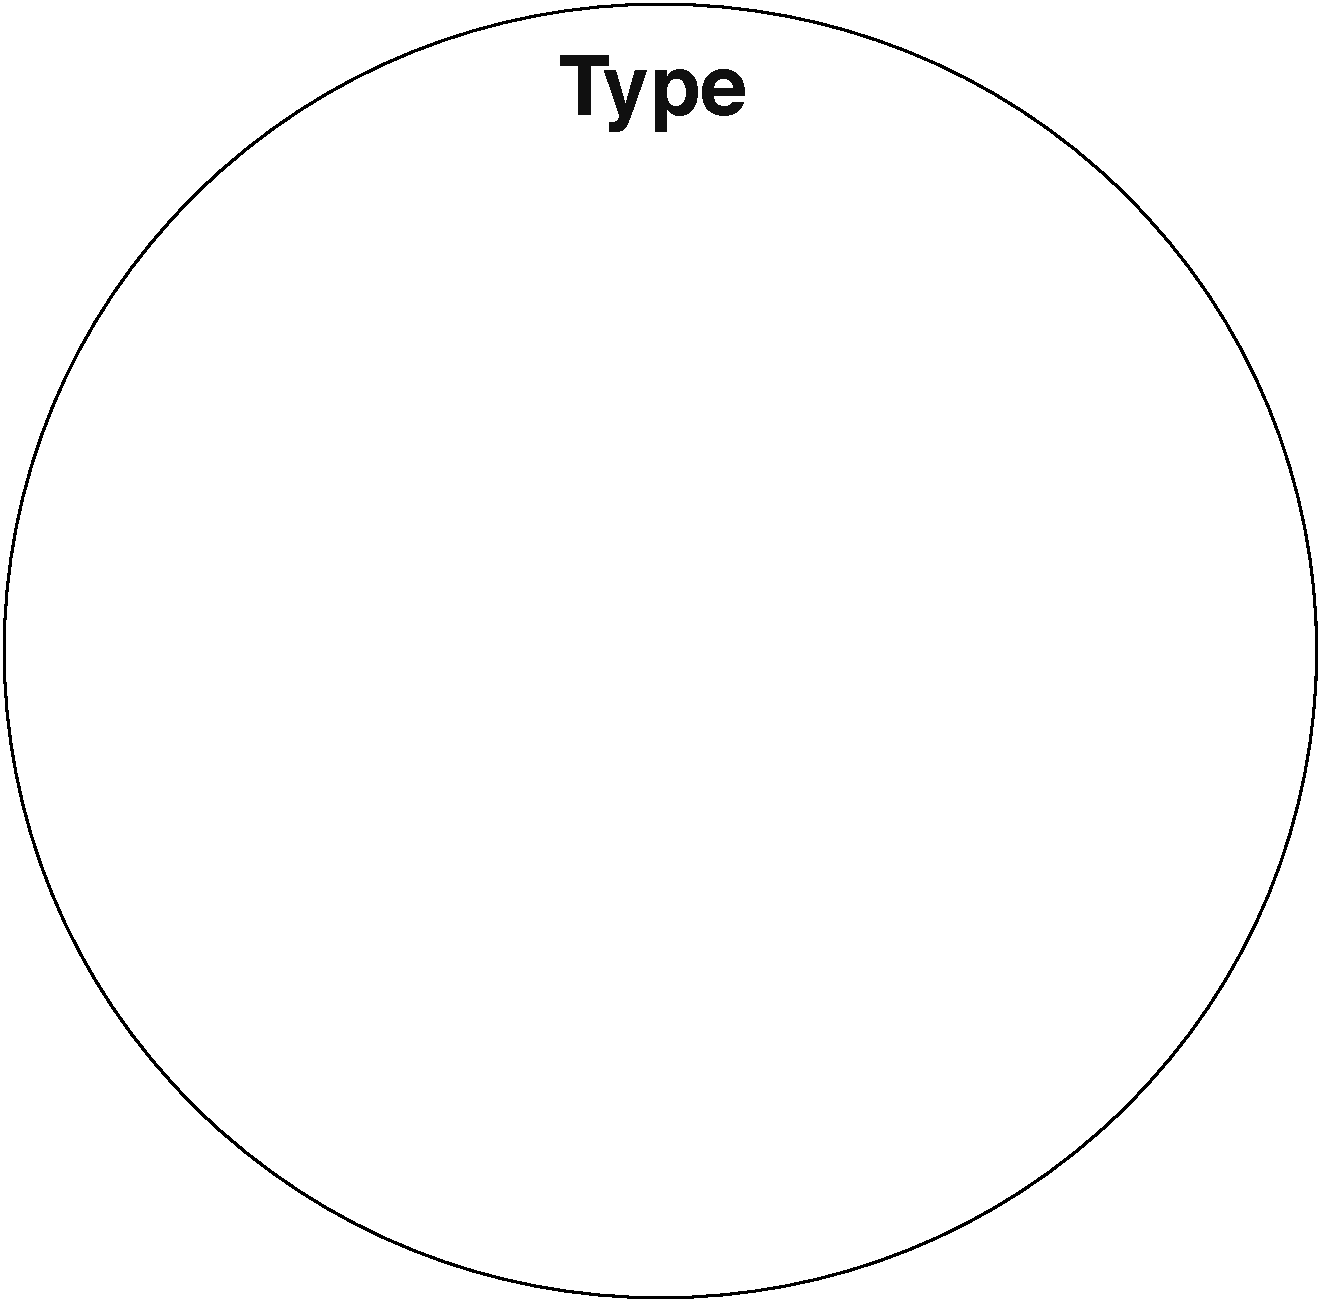
\includegraphics[width=2.5in]{universe-empty.pdf}
  \end{center}
\end{frame}

\begin{frame}
  \frametitle{Universes \`a la Tarski}
  \begin{center}
    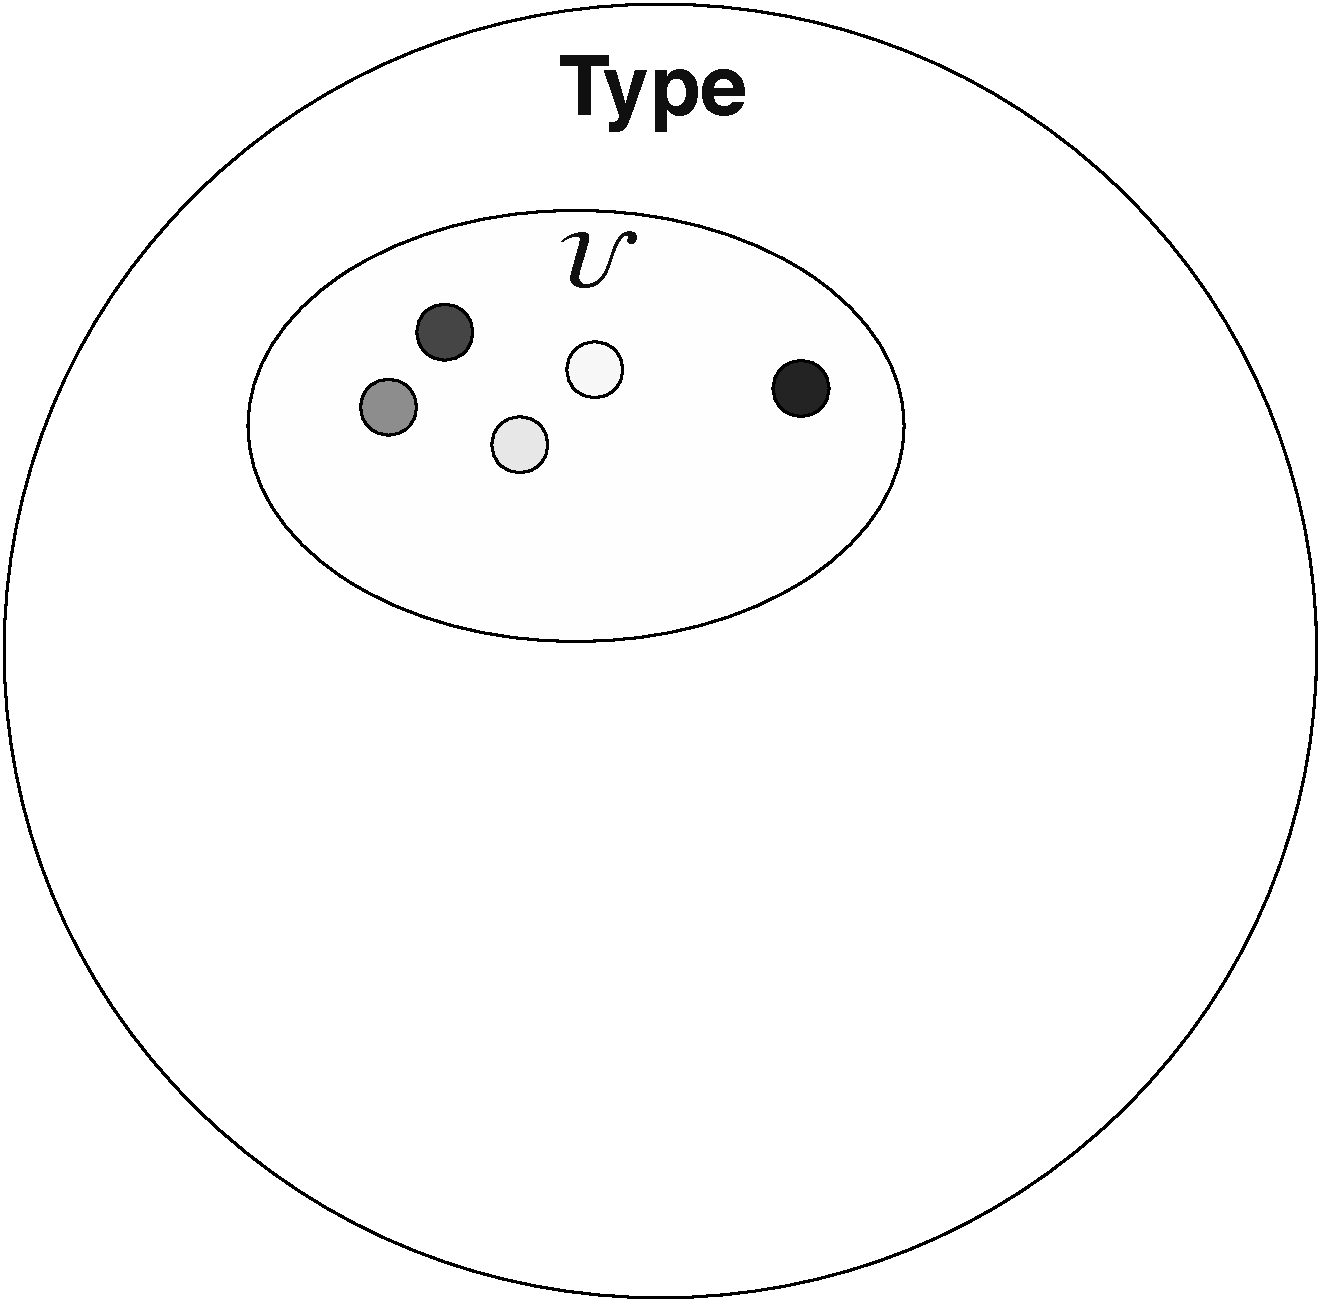
\includegraphics[width=2.5in]{universe-embedded.pdf}
  \end{center}
\end{frame}

\begin{frame}
  \frametitle{Universes \`a la Tarski}
  \begin{center}
    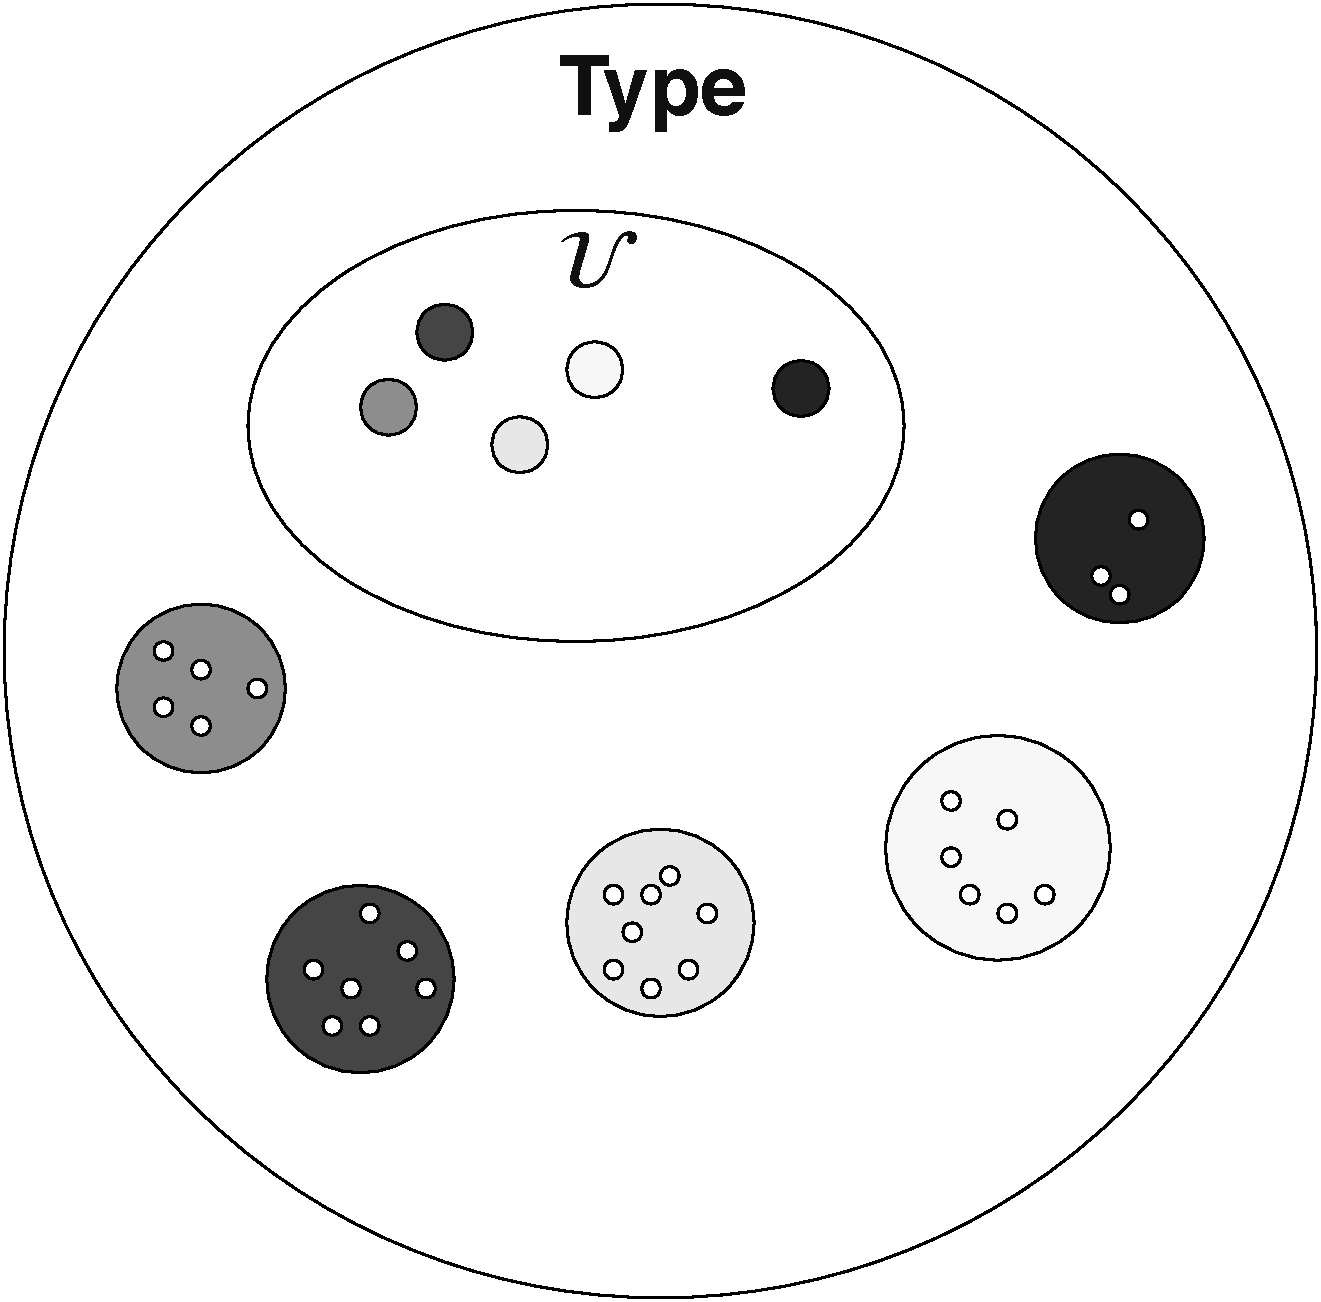
\includegraphics[width=2.5in]{universe-populated.pdf}
  \end{center}
\end{frame}

\begin{frame}
  \frametitle{Universes \`a la Tarski}
  \begin{center}
    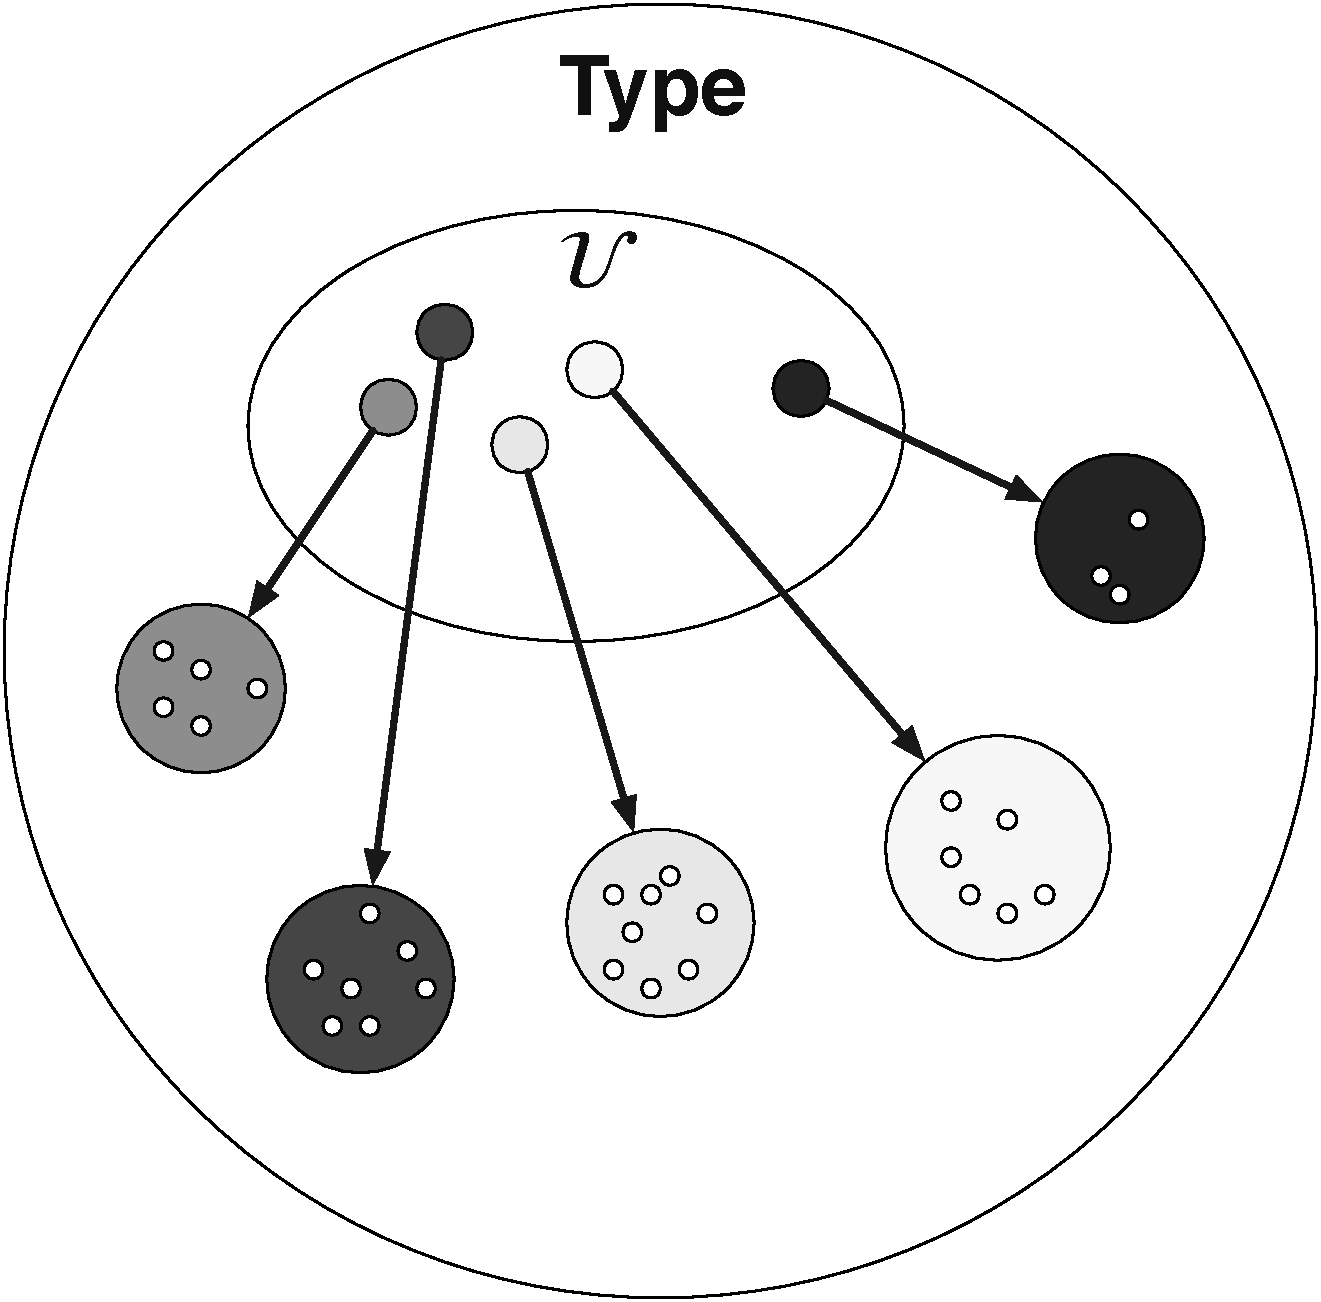
\includegraphics[width=2.5in]{universe-interpretation.pdf}
  \end{center}
\end{frame}

\begin{frame}
  \frametitle{An Example Universe}
  \pause
  Let $\mathcal{F}$ be the universe of finite sets:
  \pause
  \begin{itemize}
    \item Statics:
      \pause
      \[
        \infer{\mathcal{F} : \mathbf{Type}}{}
        \qquad
        \pause
        \infer{\textsf{fin}(n; t) : \mathcal{F}}{n : \mathbb{N} & t:\mathcal{F}}
        \qquad
        \pause
        \infer{\llbracket s \rrbracket_\mathcal{F} : \mathbf{Type}}{s : \mathcal{F}}
      \]
      \pause
    \item Dynamics:
      \pause
      \[
        \infer{
          \llbracket\textsf{fin}(n; t)\rrbracket_\mathcal{F} \leadsto \textsf{rec}_\mathbb{N}[n](T; T\times -)
        }{
          \llbracket t\rrbracket_\mathcal{F} \leadsto T
        }
      \]
  \end{itemize}
\end{frame}

\begin{frame}
  \frametitle{A Universe of Keys}
  \pause
  The $\mathtt{s ::: k}$ notion of \textbf{keys} we gave earlier is a degenerate special case of a universe of \textbf{codes}.
  \pause
  \begin{itemize}
     \item Such universes are \emph{closed}
     \pause
     \item ...and that's a good thing
  \end{itemize}
\end{frame}

\begin{frame}
  \frametitle{A Universe of Keys}
  \begin{itemize}
    \item Statics:
    \pause
      \[
        \infer{\mathcal{K}:\textbf{Type}}{}
        \pause
        \qquad
        \infer{k:::t : \mathcal{K}}{k:\text{String} & t : \textbf{Type}}
      \]
    \pause
    \item Dynamics:
    \pause
      \[
        \infer{\llbracket k:::t\rrbracket_\mathcal{K}\leadsto t}{}
      \]
  \end{itemize}
\end{frame}

\section{Type-Theoretic Records \& Sums}

\begin{frame}
  \frametitle{Records as Products}
  \pause
  \only<2,3>{
    Records: the product of the image of $\llbracket-\rrbracket_\mathcal{U}$ in $\mathbf{Type}$ restricted to a subset of the domain.
  }
  \only<4>{
    \begin{center}
      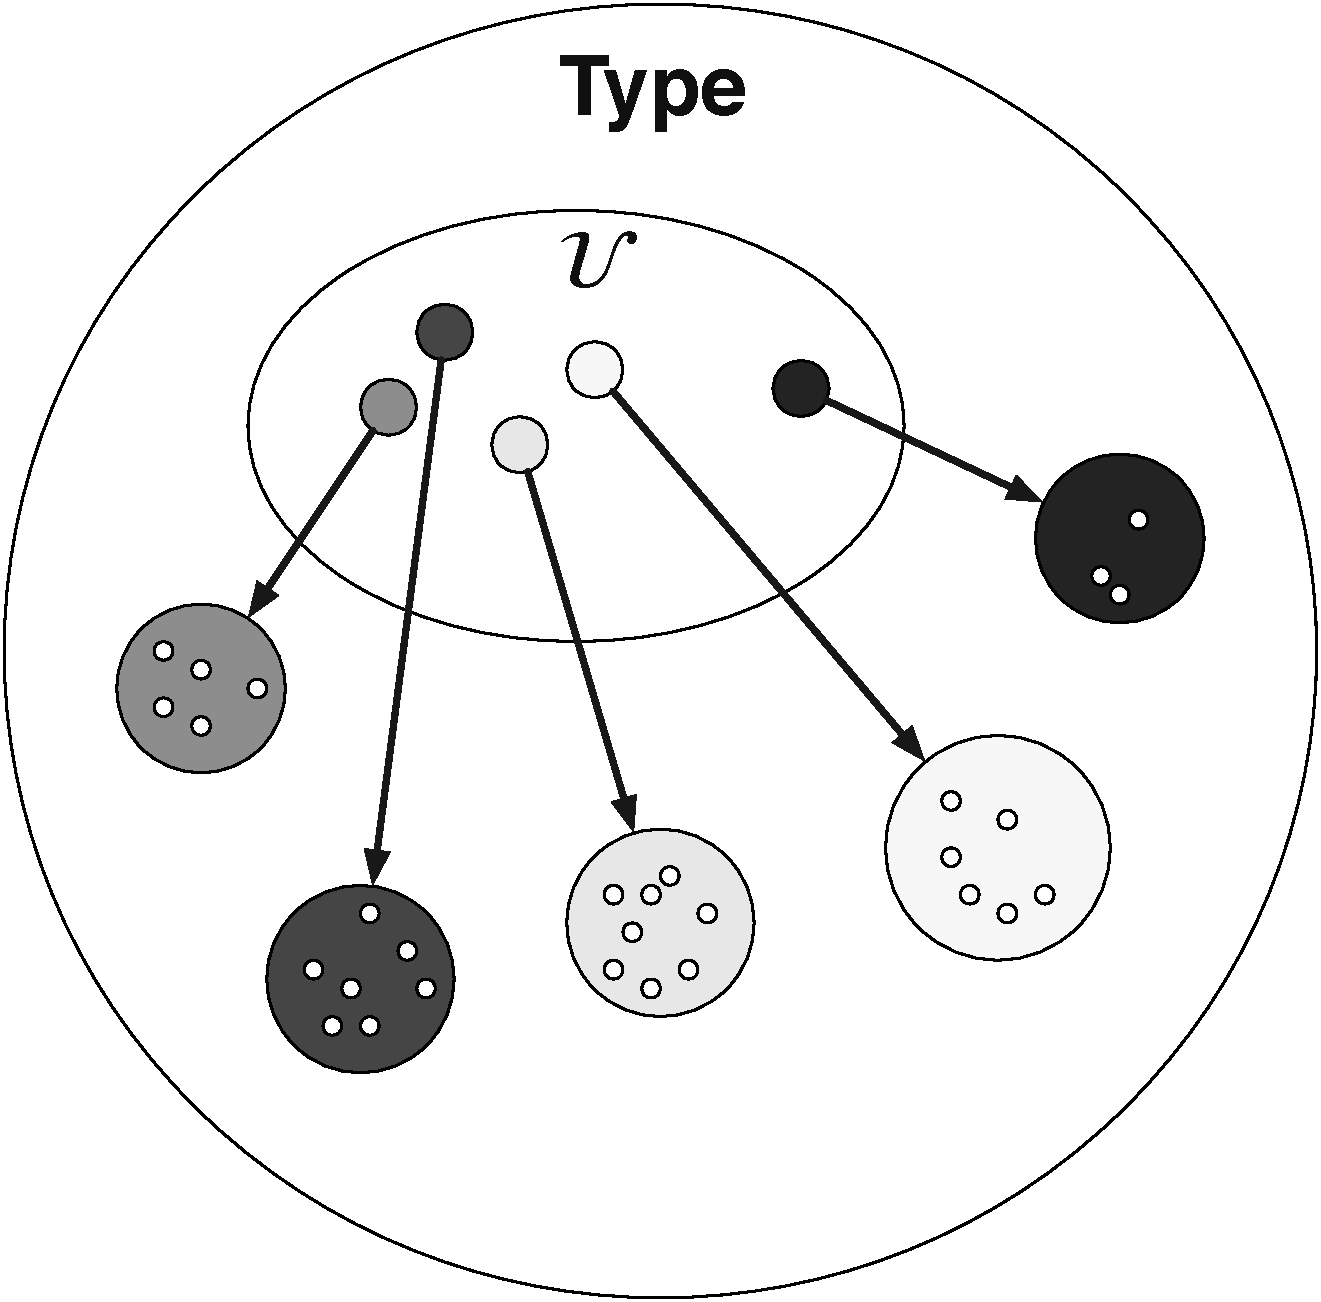
\includegraphics[width=2.5in]{universe-interpretation.pdf}
    \end{center}
  }
  \only<5>{
    \begin{center}
      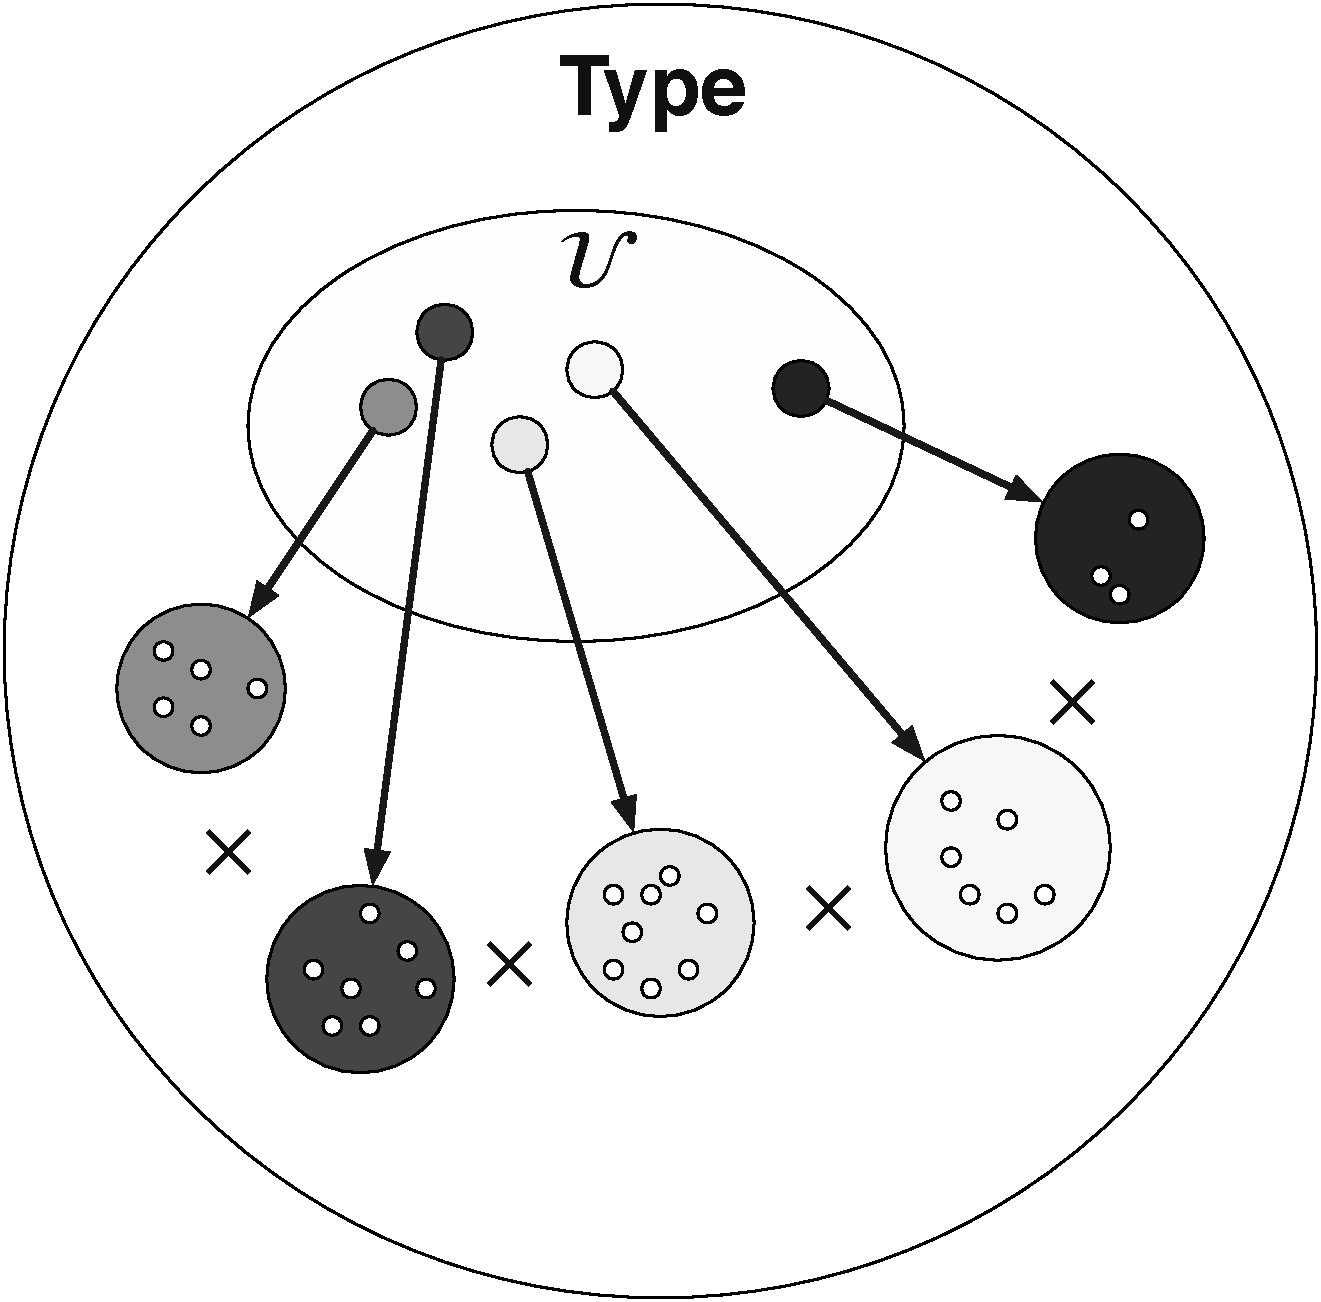
\includegraphics[width=2.5in]{universe-product.pdf}
    \end{center}
  }
  \only<3,6>{
    \[
      \mathsf{record}_\mathcal{U} \leadsto
        \sum_{\mathcal{V}:\mathbf{Type}}
        \sum_{i:\mathcal{V}\hookrightarrow\mathcal{U}}
        \prod_\mathcal{V} \llbracket-\rrbracket_\mathcal{U}\circ i
    \]
  }
\end{frame}

\begin{frame}
  \frametitle{Example Record}
  \[
    \begin{aligned}
      \mathsf{record}_\mathcal{U} &\leadsto
        \sum_{\mathcal{V}:\mathbf{Type}}
        \sum_{i:\mathcal{V}\hookrightarrow\mathcal{U}}
        \prod_\mathcal{V} \llbracket-\rrbracket_\mathcal{U}\circ i \\\\ \pause
      \mathcal{U} &\leadsto \{ \mathsf{`bool}, \mathsf{`int} \}\\ \pause
      \llbracket\mathsf{`bool}\rrbracket_\mathcal{U} &\leadsto \mathbf{2}\\ \pause
      \llbracket\mathsf{`int}\rrbracket_\mathcal{U} &\leadsto \mathbb{Z}\\\\ \pause
      ex &: \mathsf{record}_\mathcal{U}\\ \pause
      ex &\leadsto \langle\mathcal{U},\lambda x. x, \{ \mathsf{`bool}\mapsto \mathbf{1}_1; \mathsf{`int}\mapsto 34 \}\rangle
    \end{aligned}
  \]
\end{frame}

\begin{frame}
  \frametitle{Corecords as Sums}
  \pause
  \only<2,3>{
    Corecords (extensible variants): the sum of the image of $\llbracket-\rrbracket_\mathcal{U}$ in $\mathbf{Type}$.
  }
  \only<4>{
    \begin{center}
      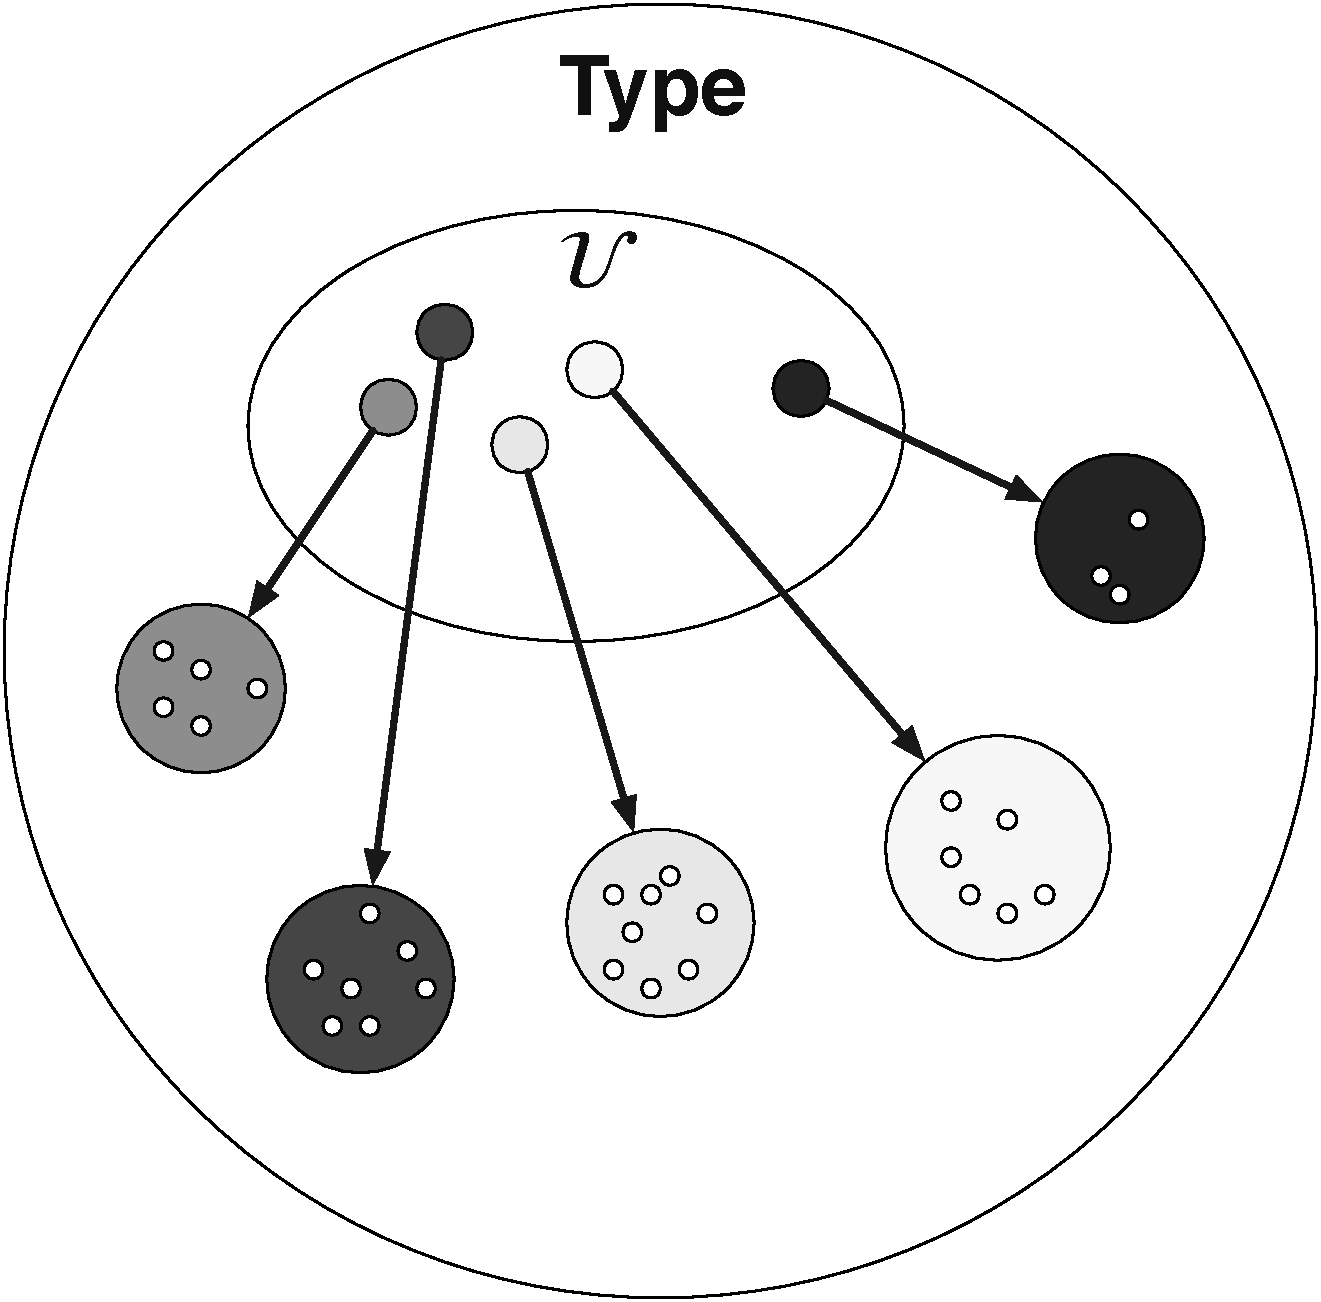
\includegraphics[width=2.5in]{universe-interpretation.pdf}
    \end{center}
  }
  \only<5>{
    \begin{center}
      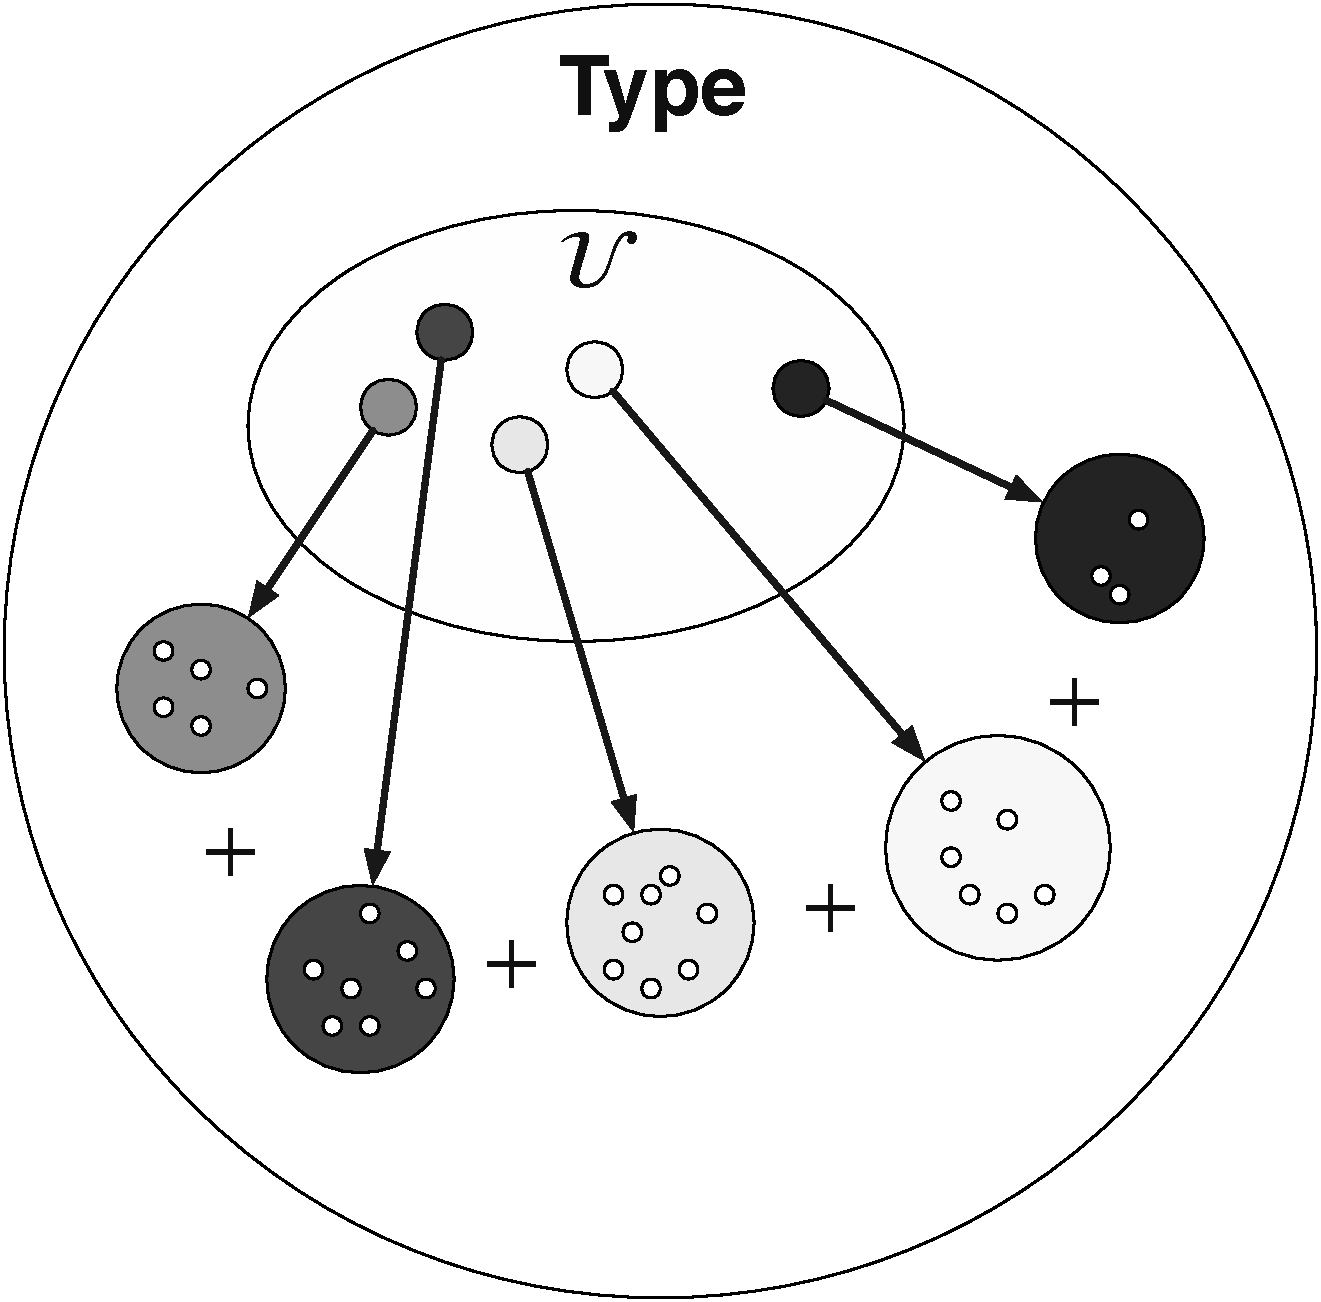
\includegraphics[width=2.5in]{universe-sum.pdf}
    \end{center}
  }
  \only<3,6>{
    \[
      \mathsf{corecord}_\mathcal{U} \leadsto
        \sum_{\mathcal{V}:\mathbf{Type}}
        \sum_{i:\mathcal{V}\hookrightarrow\mathcal{U}}
        \sum_\mathcal{V} \llbracket-\rrbracket_\mathcal{U}\circ i
    \]
  }
\end{frame}

\begin{frame}
  \frametitle{Example Corecord}
  \[
    \begin{aligned}
      \mathsf{corecord}_\mathcal{U} &\leadsto
        \sum_{\mathcal{V}:\mathbf{Type}}
        \sum_{i:\mathcal{V}\hookrightarrow\mathcal{U}}
        \sum_\mathcal{V} \llbracket-\rrbracket_\mathcal{U}\circ i\\ \pause
      \mathcal{U} &\leadsto \{ \mathsf{`bool}, \mathsf{`int} \}\\ \pause
      \llbracket\mathsf{`bool}\rrbracket_\mathcal{U} &\leadsto \mathbf{2}\\ \pause
      \llbracket\mathsf{`int}\rrbracket_\mathcal{U} &\leadsto \mathbb{Z}\\\\ \pause
      ex_1, ex_1 &: \mathsf{corecord}_\mathcal{U}\\ \pause
      ex_1 &\leadsto \langle\mathcal{U}, \lambda x.x, \mathsf{`bool}, \mathbf{1}_0\rangle\\ \pause
      ex_2 &\leadsto \langle\mathcal{U}, \lambda x.x, \mathsf{`int}, 23\rangle
    \end{aligned}
  \]
\end{frame}

\begin{frame}
  \frametitle{Doing it in Haskell}
  \pause
  \begin{itemize}
    \item Create a universe $\mathcal{U}$ at the type-level \pause
    \item Use type families to approximate $\llbracket-\rrbracket_\mathcal{U}$ \pause
    \item Parameterize \lstinline{Rec} by $\mathcal{U}$, $\llbracket-\rrbracket_\mathcal{U}$?
  \end{itemize}
\end{frame}

\begin{frame}[fragile]
  \frametitle{Records in Haskell}
  \begin{lstlisting}
    data Rec :: (|$\mathcal{U}$| -> *) -> [ |$\mathcal{U}$| ] -> * where |\pause|
      RNil :: Rec |$\llbracket-\rrbracket_\mathcal{U}$| '[] |\pause|
      (:&) :: !|$\llbracket$|r|$\rrbracket_\mathcal{U}$| -> !(Rec |$\llbracket-\rrbracket_\mathcal{U}$| rs) -> Rec |$\llbracket-\rrbracket_\mathcal{U}$| (r ': rs)
  \end{lstlisting}

  \bigskip
  \pause
  \centerline{except...}
\end{frame}

\begin{frame}[fragile]
  \frametitle{Defunctionalization to the Rescue} % TODO: add citation
  \begin{lstlisting}
    type family |$\llbracket-\rrbracket_\mathcal{U}$| (u :: |$\mathcal{U}$|) :: * |\pause|

    data TyFun :: * -> * -> * |\pause|
    type family (f :: TyFun a b -> *) |\$| (x :: a) :: b |\pause|

    data El|$_\mathcal{U}$| :: TyFun |$\mathcal{U}$| * -> * |\pause|
    type instance El|$_\mathcal{U}$| |\$| u = |$\llbracket$|u|$\rrbracket_\mathcal{U}$|
  \end{lstlisting}
\end{frame}


\begin{frame}[fragile]
  \frametitle{Defunctionalization to the Rescue}
  \begin{lstlisting}
    data Rec :: (|$\mathcal{U}$| -> *) -> [ |$\mathcal{U}$| ] -> * where
      RNil :: Rec |$\llbracket-\rrbracket_\mathcal{U}$| '[]
      (:&) :: !|$\llbracket$|r|$\rrbracket_\mathcal{U}$| -> !(Rec |$\llbracket-\rrbracket_\mathcal{U}$| rs) -> Rec |$\llbracket-\rrbracket_\mathcal{U}$| (r ': rs)
  \end{lstlisting}
\end{frame}

\begin{frame}[fragile]
  \frametitle{Defunctionalization to the Rescue}
  \begin{lstlisting}
    data Rec :: (TyFun |$\mathcal{U}$| * -> *) -> [ |$\mathcal{U}$| ] -> * where
      RNil :: Rec el|$_\mathcal{U}$| '[]
      (:&) :: !(el|$_\mathcal{U}$ \$| r) -> !(Rec el|$_\mathcal{U}$| rs) -> Rec el|$_\mathcal{U}$| (r ': rs)
  \end{lstlisting}
\end{frame}

\begin{frame}[fragile]
  \frametitle{Recovering HList}\pause
  \begin{lstlisting}
    data Id :: TyFun * * -> *|\pause|
    type instance Id |\$| t = t|\pause|

    type HList rs = Rec Id rs|\pause|

    ex :: HList [Int, Bool, String] |\pause|
    ex = 34 :& True :& "vinyl" :& RNil
  \end{lstlisting}
\end{frame}

\begin{frame}[fragile]
  \frametitle{Corecords in Haskell}\pause
  \[
    \mathsf{corecord}_\mathcal{U} \leadsto
      \sum_{\mathcal{V}:\mathbf{Type}}
      \sum_{i:\mathcal{V}\hookrightarrow\mathcal{U}}
      \sum_\mathcal{V} \llbracket-\rrbracket_\mathcal{U}\circ i
  \]
  \pause
  \begin{lstlisting}
    data CoRec :: (TyFun |$\mathcal{U}$| * -> *) -> [ |$\mathcal{U}$| ] -> * where |\pause|
      (:>) :: r :E rs => !(Sing r) -> !(el|$_\mathcal{U}$ \$| r) -> CoRec el|$_\mathcal{U}$| rs |\pause|

    ex|$_1$|, ex|$_2$| :: CoRec Id [Bool, String]|\pause|
    ex|$_1$| = SBool :> True |\pause|
    ex|$_2$| = SString :> "vinyl" |\pause|
  \end{lstlisting}
\end{frame}

\begin{frame}[fragile]
  \frametitle{Corecords in Haskell}\pause
  \begin{lstlisting}
    ex|$_1$| = SBool :> True |\pause|
    ex|$_2$| = SString :> "vinyl" |\pause|

    ex|$_1$| :: Bool :E rs => CoRec Id rs|\pause|
    ex|$_2$| :: String :E rs => CoRec Id rs|\pause|

    f :: (Bool :E rs, String :E rs) =>
       CoRec Id rs -> Maybe String |\pause|
    f (SBool :> b) = Just ("bool: " ++ show b) |\pause|
    f (SString :> s) = Just ("string: " ++ s) |\pause|
    f (_ :> _) = Nothing

  \end{lstlisting}
\end{frame}
\end{document}

